\documentclass[12pt,a4paper,titlepage]{article}
\usepackage[utf8]{inputenc} % para poder colocar acentos e caracteres especiais
\usepackage[portuguese]{babel}
\usepackage{graphicx} % Permite inserir e manipular imagens
\usepackage{fancyhdr} % 
\usepackage{caption}
\usepackage{comment}
\usepackage{geometry} % Permite definir facilmente margens e o layout da página
\usepackage{setspace} % Permite alterar o espaçamento entre linhas
\usepackage{titlesec} % Permite personalizar os títulos de secções e subseções
\usepackage[hidelinks]{hyperref} % Ativa links clicáveis no PDF
\usepackage{multicol} % coloca isto no preâmbulo


% Configuração do listings (paraexcertos de código)
\usepackage{listings}
\usepackage{xcolor}

\definecolor{codegreen}{rgb}{0,0.6,0}
\definecolor{codegray}{rgb}{0.5,0.5,0.5}
\definecolor{codepurple}{rgb}{0.58,0,0.82}
\definecolor{backcolour}{rgb}{0.95,0.95,0.92}
\renewcommand{\lstlistingname}{Excerto} % Colocar como excerto no pdf e não como Listing
\lstdefinestyle{mystyle}{
	backgroundcolor=\color{backcolour},   
	commentstyle=\color{codegreen},
	keywordstyle=\color{magenta},
	numberstyle=\tiny\color{codegray},
	stringstyle=\color{codepurple},
	basicstyle=\ttfamily\footnotesize,
	breakatwhitespace=false,         
	breaklines=true,                 
	captionpos=b,                    
	keepspaces=true,                 
	numbers=left,                    
	numbersep=5pt,                  
	showspaces=false,                
	showstringspaces=false,
	showtabs=false,                  
	tabsize=2
}
\lstset{style=mystyle}
% Ensinar o listings UTF-8
\lstset{
	extendedchars=true,
	literate=
	{á}{{\'a}}1 {é}{{\'e}}1 {í}{{\'i}}1 {ó}{{\'o}}1 {ú}{{\'u}}1
	{Á}{{\'A}}1 {É}{{\'E}}1 {Í}{{\'I}}1 {Ó}{{\'O}}1 {Ú}{{\'U}}1
	{à}{{\`a}}1 {è}{{\`e}}1 {ì}{{\`i}}1 {ò}{{\`o}}1 {ù}{{\`u}}1
	{À}{{\`A}}1 {È}{{\'E}}1 {Ì}{{\`I}}1 {Ò}{{\`O}}1 {Ù}{{\`U}}1
	{â}{{\^a}}1 {ê}{{\^e}}1 {î}{{\^i}}1 {ô}{{\^o}}1 {û}{{\^u}}1
	{Â}{{\^A}}1 {Ê}{{\^E}}1 {Î}{{\^I}}1 {Ô}{{\^O}}1 {Û}{{\^U}}1
	{ã}{{\~a}}1 {õ}{{\~o}}1 {Ã}{{\~A}}1 {Õ}{{\~O}}1
	{ç}{{\c c}}1 {Ç}{{\c C}}1
}

% Page setup
\geometry{margin=2.5cm}
\setstretch{1.5}
\pagestyle{fancy}
\fancyhf{}
\rhead{\thepage}
\lhead{Escola Superior de Tecnologia e Gestão}

% Title formatting
\titleformat{\section}{\large\bfseries}{\thesection}{1em}{}
\titleformat{\subsection}{\normalsize\bfseries}{\thesubsection}{1em}{}

\begin{document}

% Title Page
\begin{titlepage}
    \centering
    
\includegraphics[width=15cm]{imagens/estg_logo.png}\par\vspace{0.9cm} % 
    \scshape % Small caps for the institution name
    
    \rule{\textwidth}{1pt}\vspace{0.4cm} % Horizontal line
    {\Huge \bfseries Lakehouse para Análise Clínica \par}
    {Tecnologias Escaláveis para Análise de Dados\par}
    \vspace{0.4cm}\rule{\textwidth}{1pt}\par
    \vspace{2cm}
    
    \Large Mestrado em Engenharia Informática \par
    \vspace{4cm}

    \normalsize
    \textbf{Grupo 7} \par
    Diogo Pereira – 8200594 \par
    Duarte Sampaio – 8190553 \par
    Hugo Guimarães – 8220337 \par
    Nuno Silva – 8180393
    \vfill

    \large \today
\end{titlepage}


% Indice
\tableofcontents
\newpage

% Lista de Tabelas
%\renewcommand{\listtablename}{Índice de Tabelas}
%\listoftables
%\addcontentsline{toc}{section}{Índice de Tabelas}
%\newpage



\section{Introdução} \label{sec:introducao}

\subsection{Contextualização e Tema do Projeto}
Na atualidade, as instituições de saúde geram volumes massivos de dados por cada caso cirúrgico, que frequentemente acabam por permanecer isolados em diferentes silos. Este projeto desenvolve-se em torno da Empresa Y, uma organização de engenharia de dados focada no setor da saúde, que atua no domínio perioperatório com o objetivo de modernizar a infraestrutura de dados de grandes redes hospitalares.

A plataforma integra três fontes independentes: informação clínica, parâmetros hemodinâmicos e resultados laboratoriais. Contudo, a análise destes dados esbarra em sérios problemas de qualidade, nomeadamente ruído e artefactos nos sinais vitais de alta frequência, bem como timestamps assíncronos e valores nulos nos exames laboratoriais. Para resolver esta fragmentação, propõe-se a implementação de uma arquitetura Lakehouse moderna (assente em MinIO, Apache Iceberg, Trino e Flyte). Esta solução ingere e processa os dados através das camadas Bronze, Silver e Gold, garantindo a qualidade necessária para suportar modelagem preditiva e tomada de decisão.

\subsection{Objetivos do Trabalho}
O objetivo central deste trabalho prático é simular de forma realista o ciclo de vida de construção e operação de uma plataforma analítica escalável orientada a produtos de dados. Para tal, desenhou-se uma solução end-to-end que aplica os conceitos de data engineering e machine learning, assegurando a separação entre computação e armazenamento.

O projeto visa implementar pipelines orquestrados de forma reprodutível e tolerante a falhas, aplicar estratégias de otimização no processamento dos dados e garantir a qualidade da informação servida através da definição de contratos de dados rigorosos.

\subsection{Estrutura do Relatório}
Para além desta secção introdutória, o presente relatório encontra-se estruturado em cinco capítulos adicionais:
\begin{itemize}
	\item \textbf{Capítulo 2 - Definição do Problema:} Detalha os desafios inerentes aos dados médicos de alta frequência e especifica os produtos de dados propostos como solução.
	\item \textbf{Capítulo 3 - Arquitetura do Lakehouse:} Apresenta a \textit{stack} tecnológica utilizada, o modelo \textit{Medallion} (Bronze, Silver e Gold) e a forma como os \textit{workflows} foram orquestrados no Flyte.
	\item \textbf{Capítulo 4 - Governança e Garantia de Qualidade:} Explora a implementação de Contratos de Dados (Data Contracts) e a estratégia de quarentena (\textit{Dead Letter Queue}) para assegurar a fiabilidade da informação.
	\item \textbf{Capítulo 5 - Visualização de Dados:} Descreve o consumo analítico das tabelas Gold via motor SQL e a sua consequente visualização em \textit{dashboards} clínicos e operacionais no Grafana.
\end{itemize}

\newpage

\section{Definição do Problema} \label{sec:definicao_problema}

\subsection{Problema a Resolver} \label{subsec:problema_a_resolver}
A monitorização contínua em ambiente perioperatório (recorrendo ao VitalDB) gera um fluxo de dados de alta velocidade (frequentemente com múltiplos registos por segundo). O principal problema reside na extrema suscetibilidade destes sensores a artefactos mecânicos (movimentos do paciente, desconexão de cabos) e eletrónicos, resultando em falsos positivos, dados ausentes e flutuações irreais (ruído). Adicionalmente, o cruzamento deste fluxo contínuo com dados pontuais assíncronos (como exames laboratoriais) cria desafios complexos de alinhamento temporal e integração analítica, impossibilitando uma tomada de decisão médica fiável em tempo real se a informação não for devidamente validada e contextualizada.

\subsection{Produtos de Dados} \label{subsec:produtos_dados}
Para dar resposta às necessidades analíticas e operacionais do hospital descritas na secção anterior, a arquitetura disponibiliza quatro \textit{Data Products} distintos na camada Gold:

\begin{itemize}
	\item \textbf{Qualidade e Janela de Visualização dos Sinais Vitais:} Converte os dados da camada silver e gera agregações por janelas temporais para monitorizar a qualidade dos sensores e análise clínica exploratória.
	\begin{itemize}
		\item \textit{Pergunta Analítica:} Qual é a disponibilidade dos sensores ao longo da cirurgia e qual o comportamento médio dos sinais em janelas temporais fixas?
		\item \textit{Consumidor:} \textit{Dashboards} de monitorização clínica e auditoria da qualidade dos dados.
	\end{itemize}
	
	\item \textbf{Avaliação de Impacto Laboratorial (Pré vs. Pós-Operatório):} Combina os resultados laboratoriais com o histórico clínico e demográfico dos pacientes para avaliar a variância bioquímica e o desgaste fisiológico decorrentes do stress cirúrgico.
	\begin{itemize}
		\item \textit{Pergunta Analítica:} Qual a magnitude da variação dos marcadores bioquímicos críticos no período pós-operatório imediato, estratificada por especialidade médica e género?
		\item \textit{Consumidor:} \textit{Dashboard} interativo de suporte à decisão clínica e executiva (desenvolvido em Streamlit), focado na monitorização e exploração visual de tendências populacionais.
	\end{itemize}
	
	\item \textbf{Registo de Qualidade do Sensor e Anomalias de Dados:} Um produto focado na fiabilidade da infraestrutura. Avalia a qualidade do equipamento em tempo real, impondo contratos de dados rigorosos e fornecendo uma classificação final de saúde (\textit{Health Grade}) para cada dispositivo.
	\begin{itemize}
		\item \textit{Métricas:} Taxas de nulos na janela ativa, deteção de anomalias temporais (sinais congelados e picos de ruído), incidência de falhas de \textit{hardware} e desvios morfológicos entre sensores paralelos (\textit{drift}).
		\item \textit{Consumidor:} Engenheiros de dados (monitorização do \textit{pipeline}) e equipa de manutenção hospitalar (manutenção preditiva).
	\end{itemize}
	
	\item \textbf{Previsor de Alocação de UCI Pós-Operatória:} Produto que alimenta um modelo de \textit{Machine Learning} supervisionado.
	\begin{itemize}
		\item \textit{Pergunta Analítica:} Qual a probabilidade de um paciente necessitar de admissão imediata na Unidade de Cuidados Intensivos (UCI) e qual o seu tempo estimado de recuperação? 
		\item \textit{Consumidor:} Administração hospitalar para pré-alocação de recursos críticos e o modelo treinado rastreado via MLFlow.
	\end{itemize}
\end{itemize}

% !TeX spellcheck = pt_PT2-PortuguesePortugal
\section{Arquitetura do Lakehouse} \label{sec:arquitetura_lakehouse}

\subsection{Arquitetura Medalhão} \label{subsec:modelo_medalhao}

Para garantir a fiabilidade, qualidade e rastreabilidade dos dados clínicos, a arquitetura de processamento adota o Modelo Medalhão (\textit{Medallion Architecture}). Este padrão de \textit{design} estrutura, representado na Figura \ref{fig:medalioarchiteture}, divide o \textit{Data Lakehouse} em três camadas lógicas de refinamento progressivo:

\begin{figure}[h!]
	\centering
	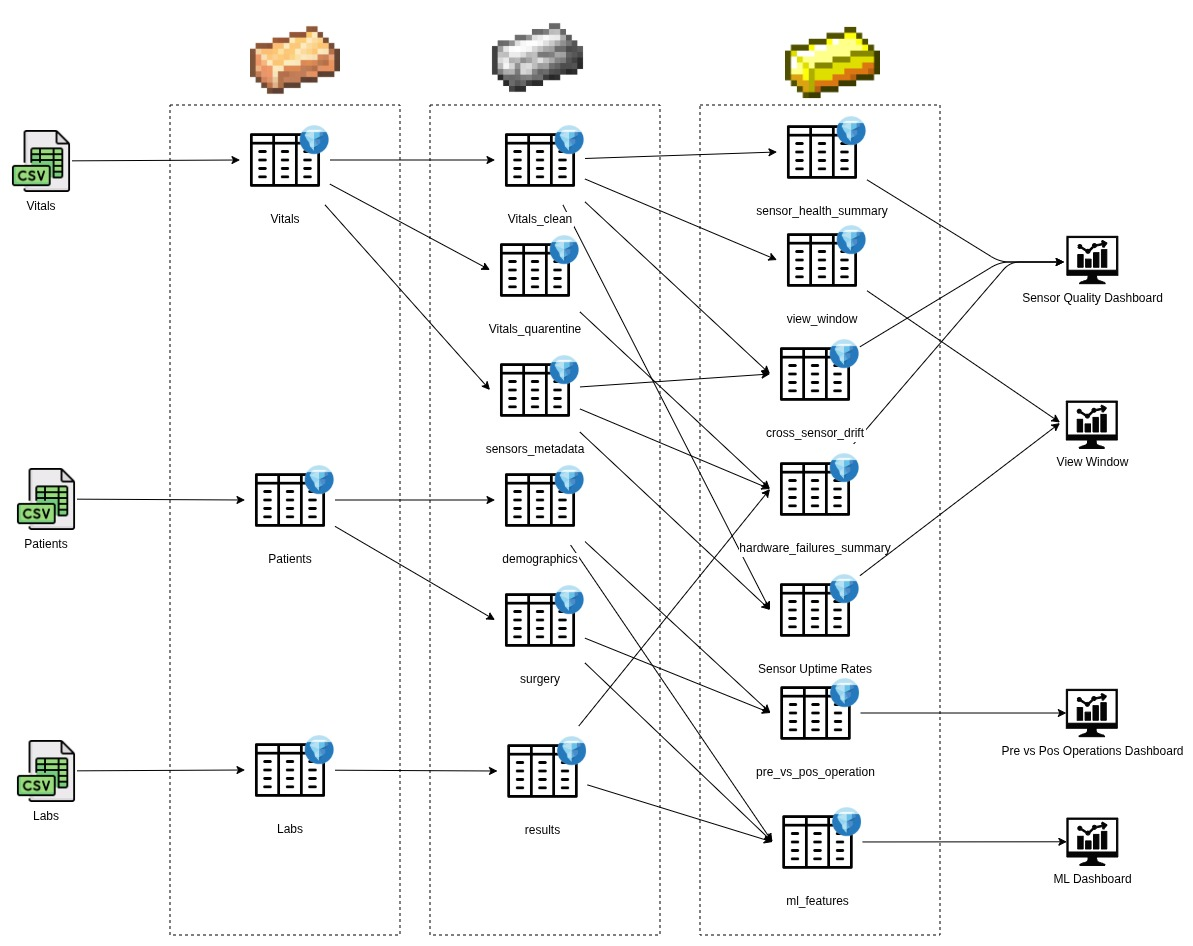
\includegraphics[width=0.75\linewidth]{imagens/architeture.jpg}
	\caption{Representação Gráfica da Arquitetura Medalhão}
	\label{fig:medalioarchiteture}
\end{figure}

\begin{itemize}
	\item \textbf{Camada \textit{Bronze} (Raw):} Atua como a zona de aterragem dos dados. Armazena a informação em estado bruto e imutável, preservando o histórico exato gerado pelos sistemas de origem hospitalar (registos de admissão, resultados laboratoriais e demografia). Os dados csv,  para entrarem nesta camada, primeiro precisam de ser convertidos para o formato \textit{parquet} e \textit{iceberg}.
	
	\item \textbf{Camada \textit{Silver} (Cleansed):} Focada na higienização e conformidade. Nesta camada, os dados brutos são filtrados, padronizados e cruzados. Registos inválidos são tratados e as entidades clínicas são unidas, estabelecendo uma base de dados fiável e relacional (ex: associação do perfil do paciente aos seus exames pré e pós-operatórios).
	
	\item \textbf{Camada \textit{Gold} (Curated):} A camada de consumo analítico. Contém dados altamente refinados e agregados, modelados especificamente para responder às necessidades de negócio. É aqui que reside as tabelas finais, que fornece as métricas pré-calculadas diretamente nos \textit{dashboards}, garantindo máxima performance de leitura.
\end{itemize}


\subsection{Orquestração de Pipelines} \label{subsec:orquestracao_pipelines}

A automatização e gestão dos fluxos de dados (\textit{data pipelines}) são asseguradas pelo \textbf{Flyte}, uma plataforma de orquestração distribuída e tolerante a falhas. O Flyte, embora permita estruturar a lógica de processamento através de Grafos Acíclicos Dirigidos (DAGs), foi impossível executar em modo \textit{"Remote"}, funcionando apenas em modo \textit{"Local"} o que, embora constrangedor, é perfeitamente funcional.

Nesta solução, o \textit{Orquestrator} é responsável por coordenar a transição da informação através do Modelo Medalhão. Ele garante que as tarefas de ingestão (\textit{Bronze}), higienização e cruzamento relacional (\textit{Silver}) e, finalmente, a agregação de métricas clínicas (\textit{Gold}) são executadas com a precedência correta. O uso do Flyte assegura não só a reprodutibilidade dos \textit{workflows}, mas também a robustez do sistema, permitindo a monitorização contínua e a reexecução isolada de tarefas em caso de falhas na infraestrutura.

\section{Governança e Garantia de Qualidade} \label{sec:governanca_garantia_qualidade}

\subsection{Padrão de Data Contracts} \label{subsec:padrao_data_products}
Para garantir a fiabilidade da plataforma, adotou-se uma abordagem baseada em \textit{Data Contracts}, seguindo as especificações do \textit{Open Data Contract Standard} (ODCS). Em vez de embutir validações no código, a estrutura, semântica e regras de negócio de cada tabela foram colocadas em ficheiros yaml. Estes contratos definem a tipagem esperada e restrições críticas (por exemplo, \texttt{age BETWEEN 0 AND 120} na tabela de demografia ou \texttt{no\_nulls(case\_id, time)} nos sinais vitais), atuando simultaneamente como documentação e especificação técnica para os consumidores de cada \textit{Data Product}.

\subsection{Implementação do Quality Gate} \label{subsec:implementacao_quality_gate}
Para forçar o cumprimento dos contratos, desenvolveu-se um componente de \textit{Quality Gate} integrado diretamente no Flyte. Este avaliador em Python intercepta os \textit{DataFrames} antes da persistência dos mesmos no Lakehouse. Lendo o ficheiro YAML correspondente, traduz as regras em \textit{strings} para testes (via Pandas/PyArrow). O componente funciona sob o padrão arquitetural de \textit{Circuit Breaker}: caso os dados apresentem qualquer violação de integridade face ao contrato, a \textit{task} falha de imediato e a transação de escrita na tabela Apache Iceberg é abortada, garantindo que as camadas Silver e Gold permanecem limpas.

\subsection{Garantia de Idempotência e Operações de \textit{Upsert}} \label{subsec:garantia_idempotencia}
Para evitar duplicações e garantir consistência em reexecuções, implementou-se um mecanismo de idempotência focado em \textit{Upserts} no \textit{workflow} bronze dos pacientes. O algoritmo cruza o novo lote com a tabela Apache Iceberg via chaves primárias (ex: \texttt{caseid}, \texttt{subjectid}). Metadados técnicos (como \texttt{ingest\_time}) são ignorados na comparação para impedir atualizações causadas apenas por novos carimbos temporais. Após isolar inserções inéditas (\textit{Insert}) e detetar reais variações clínicas (\textit{Update}), o \textit{DataFrame} final é gravado numa transação ACID única (via \textit{overwrite}). Isto assegura que o \textit{Lakehouse} mantém um estado determinístico, preservando a auditoria das alterações nos \textit{logs} do orquestrador.

\subsection{Estratégia de Quarentena} \label{subsec:estrategia_quarentena}
A gestão de dados anómalos ou ruidosos (tais como falhas de hardware, valores impossíveis ou identificadores inválidos) foi implementada com base no padrão \textit{Dead Letter Queue} (DLQ). Na camada Silver, a validação e separação dos dados são realizadas em simultâneo: os registos válidos progridem para as tabelas limpas (ex: \texttt{vitals\_clean}), enquanto os registos que falham as regras de negócio são isolados em tabelas dedicadas (ex: \texttt{vitals\_quarantine}). Estas tabelas de quarentena retêm os dados originais acompanhados de uma nova coluna \texttt{error\_reason}, permitindo a auditoria contínua, o realimentar de \textit{dashboards} de manutenção técnica e a eventual re-ingestão, sem comprometer a disponibilidade dos dados saudáveis.

\subsection{Otimização Analítica e Processamento Escalonável} \label{subsec:otimizacao_queries}
Embora não tenha sido o principal foco do projeto, foram aplicados princípios de processamento escalonável (\textit{Scalable Processing}) e otimização na camada de \textit{Serving} (Trino/Grafana). O objetivo foi assegurar que o sistema cumpre os \textit{Service Level Objectives} (SLOs) de performance, minimizando o custo por execução (\textit{cost per run}) perante volumes crescentes de dados.

Um exemplo prático desta aplicação encontra-se na consulta SQL desenvolvida para alimentar o gráfico de "Distribuição de Tipos de Falha por Marca de Equipamento" no \textit{dashboard} de manutenção:

\begin{lstlisting}[language=SQL, caption={Query SQL para Distribuição de Tipos de Falha por Marca de Equipamento}, label={lst:SQL_bom}]
	WITH erros_agrupados AS (
		SELECT equipment_brand, error_reason, CAST(SUM(failure_count) AS DOUBLE) AS total_falhas 
		FROM iceberg.gold.hardware_failures_summary 
		WHERE equipment_brand IN (${marca:singlequote})
		GROUP BY equipment_brand, error_reason
	)
	SELECT 
		equipment_brand, error_reason, total_falhas,
		ROUND((total_falhas / SUM(total_falhas) OVER (PARTITION BY equipment_brand)) * 100, 2) AS pct_erro
	FROM erros_agrupados
	ORDER BY equipment_brand, pct_erro DESC
\end{lstlisting}

Esta consulta é otimizada através dos seguintes mecanismos:
\begin{itemize}
	\item \textbf{\textit{Predicate Pushdown} Prévio:} O filtro \texttt{WHERE equipment\_brand IN (...)} é aplicado logo na \textit{Common Table Expression} (CTE) inicial, reduzindo drasticamente o volume de dados a ler da tabela Iceberg antes de qualquer agregação pesada (\textit{Filter Pushdown}).
	
	\item \textbf{Gestão Eficiente de \textit{Shuffle}:} Em vez de calcular a percentagem total de falhas, forçando um cruzamento de dados (\textit{Join}) com uma tabela agregada externa, a consulta utiliza uma \textit{Window Function} (\texttt{SUM(...) OVER(PARTITION BY...)}). O uso de agregações em janela não precisa de grandes operações para movimentar os dados (\textit{shuffle-heavy}), limitando o processamento à partição específica em memória.
\end{itemize}

\section{Visualização dos Dados} \label{sec:visualizacao_dados}

\subsection{Saúde e Qualidade dos Sensores} \label{subsec:saude_qualidade_sensores}
O \textit{dashboard} de Qualidade dos Sensores foi construído no Grafana e liga-se diretamente à camada \textit{Gold} do \textit{Lakehouse} via motor SQL (Trino). A sua principal função é traduzir as milhões de leituras e anomalias filtradas num diagnóstico visual e acionável para a equipa de manutenção hospitalar. Através de \textit{scorecards} agregados, é possível monitorizar a percentagem de equipamentos com funcionamento "Excelente" e "Aceitável", bem como identificar rapidamente taxas de erro e problemas de conectividade.

A visão detalhada em formato de tabela permite à equipa técnica isolar rapidamente os componentes que apresentam "Falha Crítica" ou estado "Degradado". A avaliação é suportada por métricas concretas processadas ao segundo, como o número de picos de ruído, sinais congelados e a duração real da utilização do sensor. Esta abordagem transforma a resposta a avarias num processo de manutenção preditiva, indicando aos técnicos exatamente qual o caso clínico e o equipamento que necessitam de intervenção ou recalibração antes de comprometerem futuras cirurgias.

\begin{figure}
	\centering
	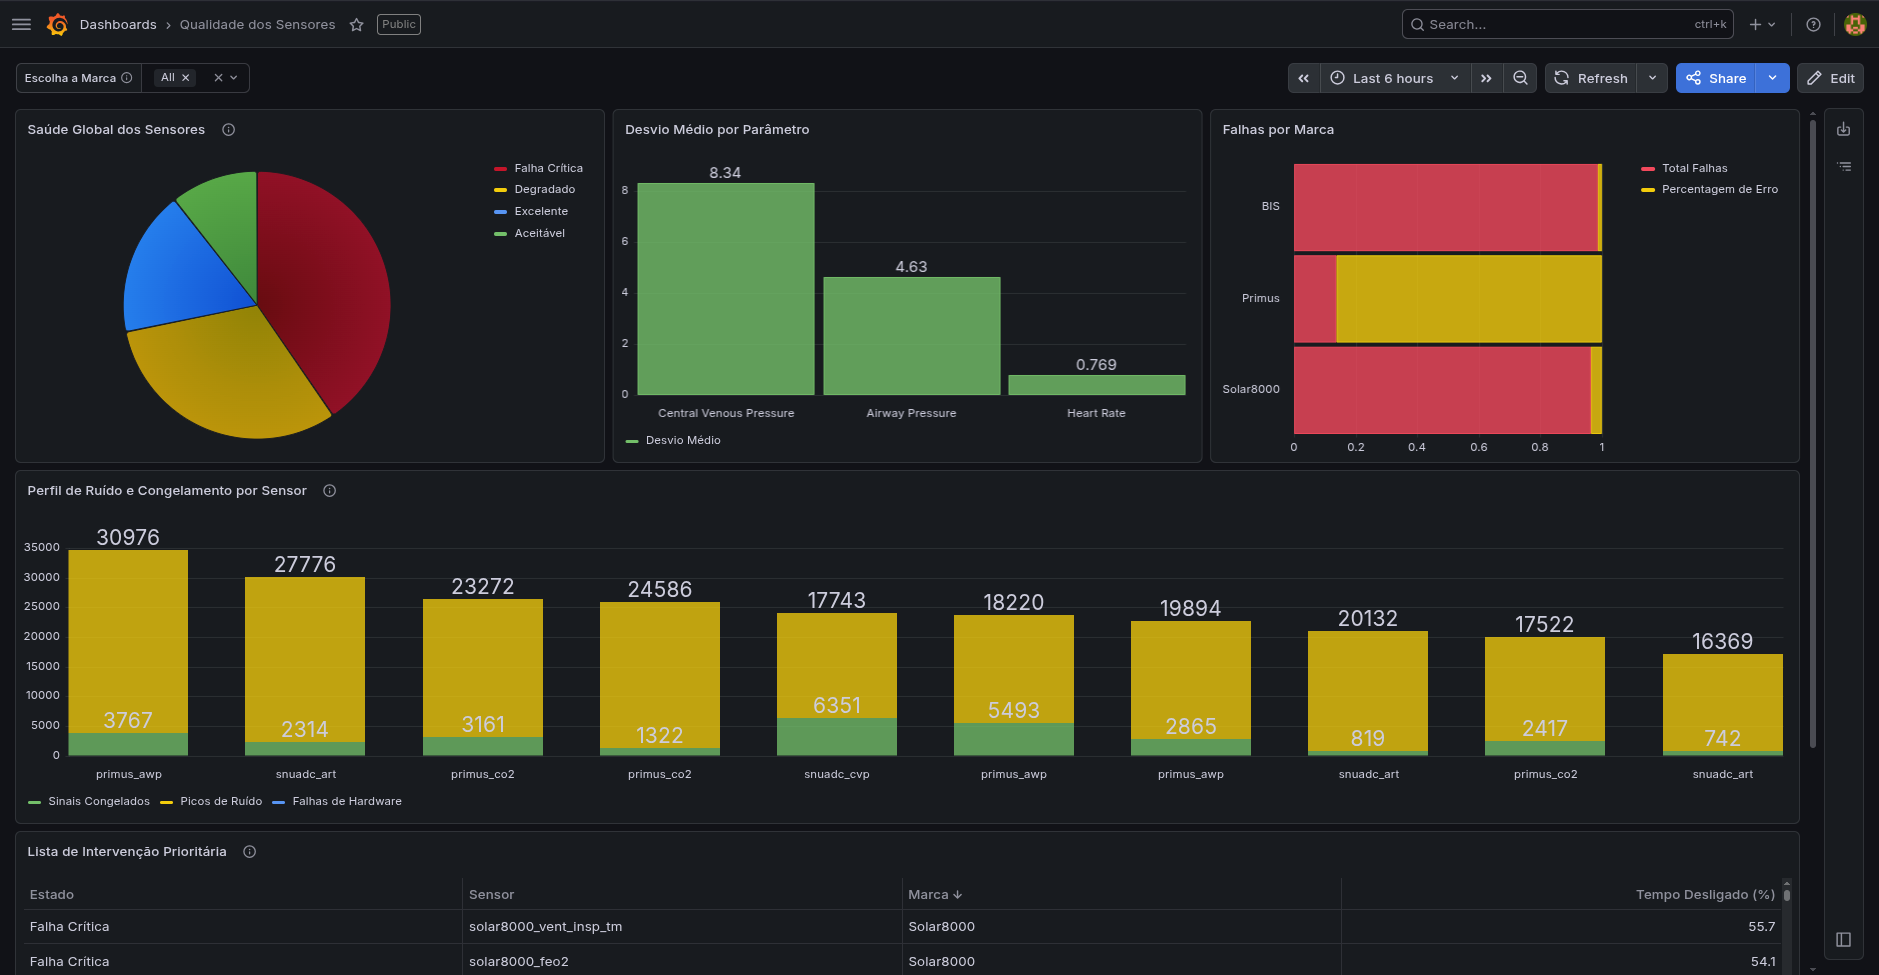
\includegraphics[width=0.7\linewidth]{imagens/qualidade_sensores_hugo}
	\caption{Dashboard Grafana de Saúde e Qualidade dos Sensores}
	\label{fig:qualidadesensoreshugo}
\end{figure}
\subsection{Pré. vs. Pós Operação} \label{subsec:pre_vs_pos_operacao}
O \textit{Dashboard} clínico pré e pós operatório permite medir o impacto e o cansaço causados pela cirurgia. Com base nos dados de todos os pacientes, o ecrã usa um gráfico \textit{Lollipop} para ajudar a equipa médica a ver rapidamente o que mudou em dezenas de análises ao sangue. Esta imagem mostra de forma clara o que desceu (linhas para a esquerda a rosa, ex: AMMO) e o que subiu ou se manteve (linhas para a direita a azul, ex: CCR ou PO2) logo a seguir à operação.

Além disso, a plataforma separa os resultados por género, usando gráficos de barras para mostrar as diferenças entre homens e mulheres. Este detalhe revela problemas que ficam escondidos quando olhamos apenas para a média geral. Por exemplo, mostra que a queda do valor de AMMO é muito mais grave nos homens.

Com a ajuda de filtros por especialidade médica e por indicador clínico, o painel transforma dados difíceis em informação clara e útil. Isto ajuda os médicos a planear melhor a recuperação de cada paciente.
\begin{figure}[h]
	\centering
	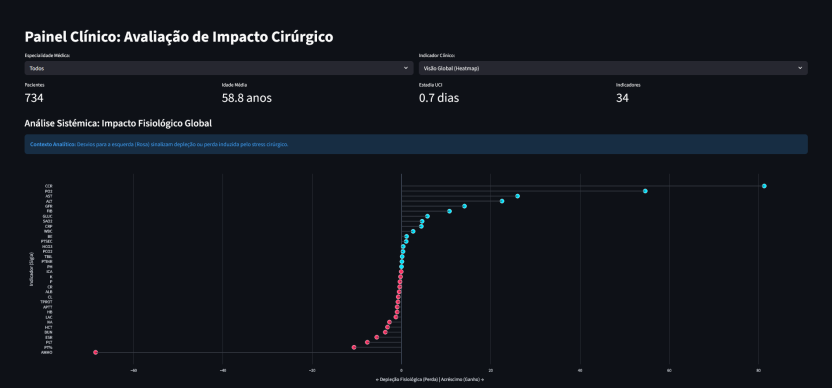
\includegraphics[width=0.7\linewidth]{imagens/pre_pos_operacao_duarte_1}
	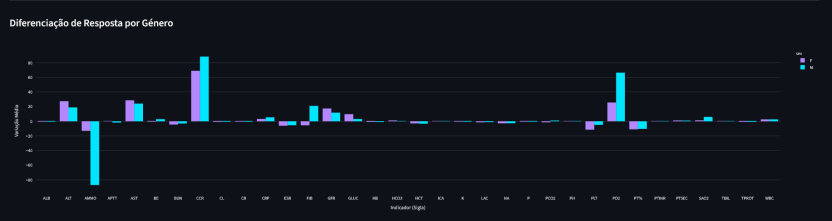
\includegraphics[width=0.7\linewidth]{imagens/pre_pos_operacao_duarte_2}
	\caption{Dashboard Streamlit Pré e Pós Operatório}
	\label{fig:preposoperacaoduarte}
\end{figure}

\subsection{Volatilidade dos Sinais Vitais} \label{subsec:volatilidade_sinais_vitais}
O dashboard desenvolvido tem como objetivo apoiar a interpretação dos sinais vitais recolhidos durante o procedimento cirúrgico, permitindo comparar o sinal bruto com o sinal suavizado e observar o efeito do processamento aplicado. A interface foi organizada em torno de filtros de cirurgia e sensor, o que possibilita ao utilizador selecionar rapidamente o contexto clínico pretendido e analisar a respetiva evolução temporal. Para melhorar a leitura dos resultados, o dashboard inclui ainda informação descritiva sobre cada sensor, como o parâmetro medido, a unidade de medida e a marca do equipamento, tornando a análise mais intuitiva e menos dependente de identificadores técnicos.

A página principal do relatório apresenta, lado a lado, o sinal antes e depois da suavização, facilitando a comparação entre a variabilidade original e a tendência subjacente após tratamento dos dados. Esta abordagem permite evidenciar a utilidade da suavização na redução de ruído e na interpretação clínica dos sinais. Além disso, a estrutura do dashboard foi pensada para ser interativo e orientada ao utilizador final, permitindo explorar os dados por cirurgia e por sensor sem necessidade de recorrer a consultas à base de dados. Desta forma, o dashboard transforma dados operacionais em informação visual mais clara, apoiando a análise exploratória e a comunicação dos resultados.

\begin{figure}[h]
	\centering
	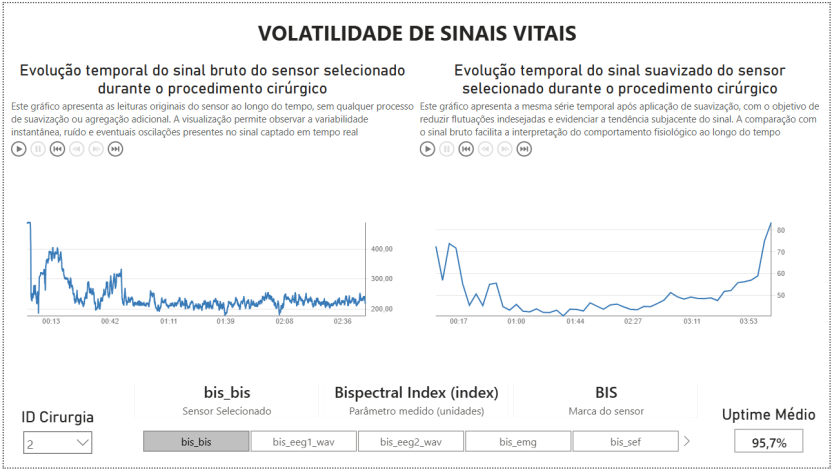
\includegraphics[width=0.7\linewidth]{imagens/volatilidade_nuno}
	\caption{Dashboard PowerBI de Volatilidade dos Sinais Vitais}
	\label{fig:volatilidadenuno}
\end{figure}

\subsection{Predições para Cuidados Intensivos}
O workflow de inferência do ICU Days Predictor foi implementado como uma pipeline do Flyte composto por quatro tarefas. Dado um ID relativo a um caso de paciente, a tarefa \textit{fetch\_case\_features} reconstrói o mesmo vetor de características utilizado durante o treino. Consultando a camada Silver, esta junta os dados demográficos do paciente (idade, sexo, IMC, score ASA) com o contexto cirúrgico (departamento, tipo de operação, abordagem, tipo de anestesia) e transforma os resultados laboratoriais pré-operatórios (hemoglobina, plaquetas, leucócitos, glicose, creatinina, albumina) numa única linha plana (flat row).

As tarefas \textit{find\_best\_regression\_model} e \textit{find\_best\_classification\_model} consultam o servidor do MLflow, classificando todas as execuções registadas na experiência \textit{ICU\_Days\_Regression} pelo menor RMSE, e na experiência \textit{ICU\_Days\_Classification} pelo maior AUC-ROC, devolvendo o URI do registo de modelos do vencedor.

Por último, a tarefa \textit{run\_predictions} carrega ambos os modelos a partir do MLflow Model Registry, aplica-os à linha de características e devolve um resultado estruturado em JSON contendo o número previsto de dias no UCI (regressão), o veredicto binário de admissão no UCI (classificação) e o valor real para comparação. Este design garante que a seleção do modelo seja sempre orientada por dados e reflita automaticamente qualquer reajuste futuro, sem a necessidade de atualizações manuais no pipeline de inferência.

\begin{figure}
	\centering
	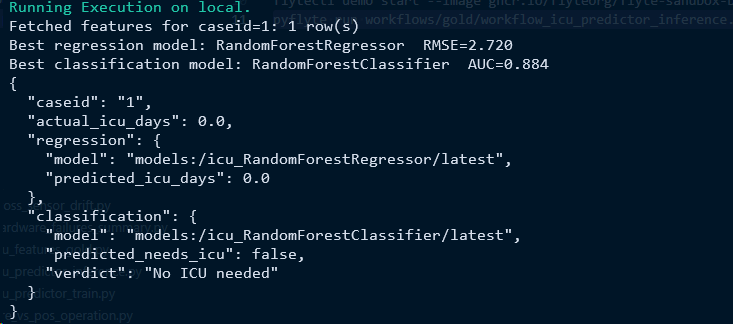
\includegraphics[width=0.7\linewidth]{imagens/predicoes_diogo}
	\caption{Output da Consola da Predição}
	\label{fig:predicoesdiogo}
\end{figure}




\end{document}
